\section{问题分析}

% 2 页
% 需要追加

受到 path2vec 模型的随机路径采样方法的启发,对于网络路由的异常检测问题,本章节将以随机游走的角度进行转化和重新阐述,将问题表述为在未知采样规则条件下的路径嵌入问题。

\subsection{问题的定义}

一般而言,在网络的异常路由检测问题上,给定的数据输入为一个网络路由表,即一个或多个路由序列 $R=\{R_1^k, R_2^k, R_3^k, ... R_n^k\}$,其中 $R^k$ 为由包含 $k$ 个不同属性的路由条目。

异常路由检测问题的目标是,在已知部分路由信息 $R_o^k$ 的条件下,通过对路由序列元素的属性进行建模,对新的路由更新信息 $R_{update}^k$ 做出异常检测。

\subsection{问题的转化}

将路由中的 AS Path 信息拆分出来后,以上的路径异常检测问题能够被转化为一个图论问题:

设序列 R 属于一个未知拓扑结构的图 $G<V,E>$,序列 R 是图 G 某种采样规则 $M$ 生成的,序列元素 $R_i<P,C>$ 包含拓扑和属性两个方面的信息,其中,P 的定义为由一系列自治系统编号 $A_i$ 组成的有序列表:$P=\{A_1, A_2, A_3, ... A_m\}$,C 被定义为一个包含标记信息的列表: $C=\{C_1, C_2, C_3,...,C_i\}$。

问题的目标被转化为,在已知部分路由信息 $R_o$ 的条件下,利用其中的 P 对图的拓扑信息进行建模,结合路由信息中的属性值 C,学习一个具有利用二者信息的模型来反应,对新的路由更新信息 $R_{update}$ 做出异常检测。

已知采样规则 M 是通过路由选择算法产生的,即 $R=f_M(G<V,E>)$,最短路径是它采样概率的最重要因素,因此问题的求解可借助某种算法 $f_R$ 去还原路由选择算法的逆变换,即 $f_R = \bar{f_M}$,因此,本文将在后续章节对路由拓扑采样的本质进行分析。

如图 \ref{c5-compare} 所示,本章描述的问题与基于随机游走的图网络嵌入算法(如 node2vec)类似,均通过采样路径获得节点对应的嵌入。与之不同的在于获取采样路径的步骤上:利用图网络度量,能够从原始数据集中采样获得逼近以某种策略为基础的随机游走路径集合,并使用与 node2vec 类似的方式进行图的表征。

\begin{figure}[h]
    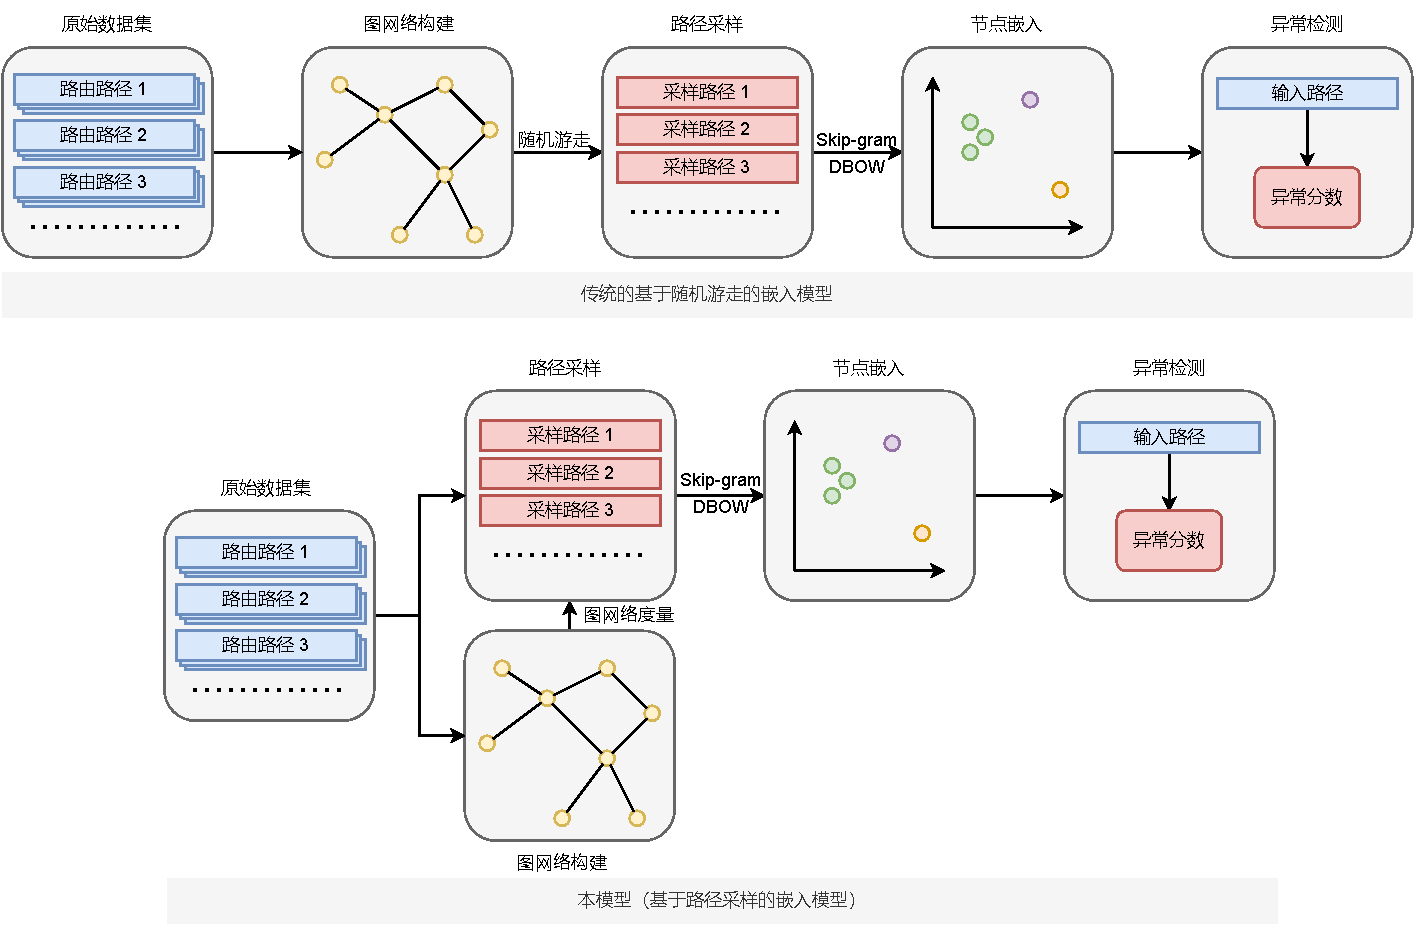
\includegraphics[width=\linewidth]{chapter/c5_images/c5-compare.pdf}
    \caption{基于随机游走的嵌入算法与本章模型的关联}
    \label{c5-compare}
\end{figure}